%\chapter{Aplicação dos Modelos de Agrupamento e Previsão em Redes Dinâmicas}
%\label{chap:modelo-agrupamento}

\section{Modelo de agrupamento ST-DBSCAN}
O modelo de agrupamento \acrshort{ST-DBSCAN} indica a formação de grupos analisando ${s}$ semanas, onde ${s}$ é configurável na aplicação, e os exibindo de acordo com a semana selecionada. Ele detecta grupos principalmente em relação à distância máxima entre os pontos no mesmo grupo e as ${s}$ semanas em análise, como demonstrado na seção \ref{stdbscan}.

\section{Modelo de agrupamento ST-IGN}
\label{sec:modelo-st-ign}
O modelo \acrshort{ST-IGN} leva em consideração as mesmas semanas analisadas que o \acrshort{ST-DBSCAN}, e além disso detecta grupos separando a \acrshort{AGM} encontrada pelo algoritmo de Kruskal. Após a execução do \acrshort{ST-IGN} tem-se a formação da \acrshort{AGM} em sub-árvores ou grupos, compostas por sub-conjuntos de arestas conexas. E finalmente, os vértices dessas arestas são agrupados utilizando o algoritmo \emph{Convex Hull}-Envoltória Convexa para a formação dos grupos de previsão. Um exemplo do resultado deste algoritmo é apresentado na figura \ref{fig:st-ign-convex}.

\begin{figure}[!ht]
	\centering	
	\Caption{\label{fig:st-ign-convex} \acrshort{ST-IGN}: Convex Hull}
	\UECEfig{}{
		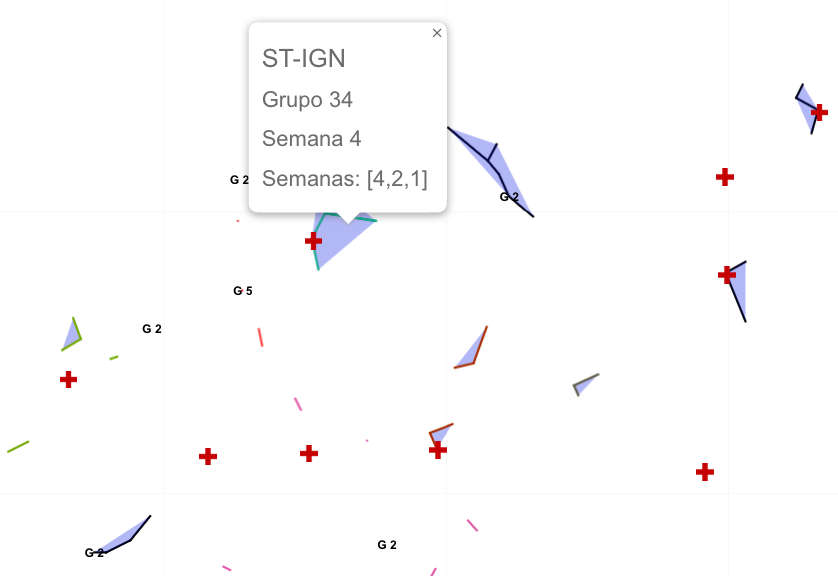
\includegraphics[width=12cm]{figuras/predicao/ST-IGN_Convex_Hull.png}
	}{
		\Fonte{Elaborado pelo autor}
	}
\end{figure}
\FloatBarrier

A separação dos grupos segue um critério de corte pré-estabelecido. Segundo \cite{simposioNeg2003}, um critério de separação deve ser inserido após uma indecidibilidade quanto à naturalidade dos grupos encontrados. Isso acontece quando a dispersão dos indivíduos está muito próxima de dois grupos naturais, confundindo com as distâncias internas entre elementos de cada grupo, resultando em que os grupos naturais sejam unidos num só grupo. Essa grande quantidade de indivíduos num grupo acarreta outro problema. Esta anomalia aparece por exemplo quando alguns dos casos de endemias na base de dados estão tão próximos (menos de 1 metro) que faz com que a função de custo da \acrshort{AGM} indique o corte nestes pontos. E com isso, praticamente descarta quase todos os pontos do grupo.

Para minimizar esse problema com grande quantidade de dados num só grupo, o modelo \acrshort{ST-IGN} implementado armazena todos os resultados da funcão de custo da \acrshort{AGM}, que indica a posição dos grupos naturais, e caso este número de cortes indique mais de que ${C}$\% de remoção de arestas, então o número anterior encontrado é utilizado, e esse processo é feito até que a condição seja satisfeita. Foi estabelecido para o número ${C}$ o valor 70 após testes no algoritmo, onde o objetivo era encontrar o máximo de grupos após o corte determinado pela função de custo.

Foram observados nos testes do algoritmo sobre os conjuntos de dados desta dissertação, que quanto menor a distância máxima entre os casos humanos, até um certo valor, maior é a quantidade de grupos encontrados sem ocorrer o problema anterior apresentado, pois no primeiro passo do algoritmo, que é encontrar a \acrshort{AGM}, alguns subgrupos menores já são formados.
A figura \ref{fig:agm} exibe um exemplo da \acrshort{AGM} gerada inicialmente pelo algoritmo \acrshort{ST-IGN}.

\begin{figure}[!ht]
	\centering	
	\Caption{\label{fig:agm} \acrshort{ST-IGN}: \acrshort{AGM} - Árvore Geradora Mínima}
	\UECEfig{}{
		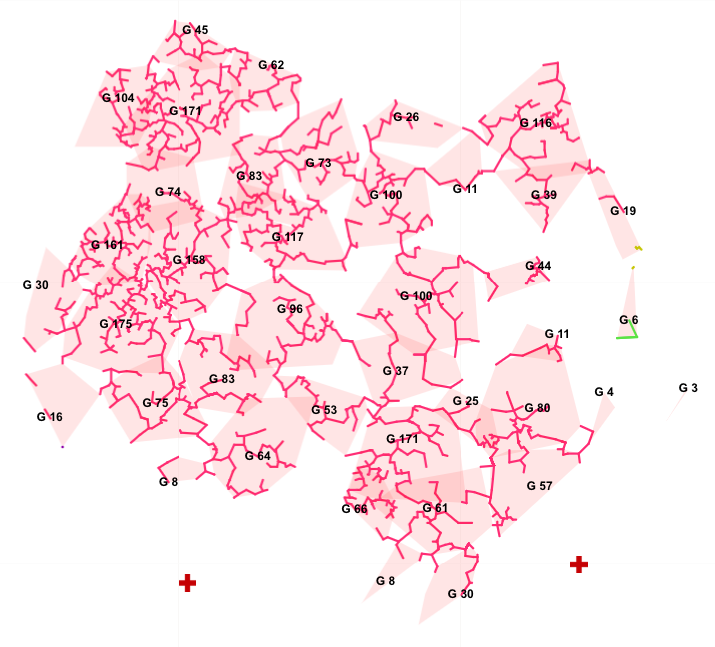
\includegraphics[width=12cm]{figuras/predicao/1000mAGM.png}
	}{
		\Fonte{Elaborado pelo autor}
	}
\end{figure}
\FloatBarrier

\section{Modelo de previsão baseado nos \emph{clusters} anteriores (centro e raio)}

Este modelo gera grupos de previsão baseados no histórico dos grupos, nos seus centros geométricos em análise e nos seus raios de acordo com a média do número de casos humanos da doença de cada grupo.

As figuras \ref{fig:stdbscan1}, \ref{fig:stdbscan2} e \ref{fig:stdbscan3} exibem os grupos formados pelo \acrshort{ST-DBSCAN}, onde os dados tomados de exemplo são os casos humanos de dengue de janeiro de 2017. A figura \ref{fig:stdbscan3} exibe também os grupos de predição formados pelo grupo 55 e 57.

\begin{figure}[!ht]
	\centering	
	\Caption{\label{fig:stdbscan1} \acrshort{ST-DBSCAN}: Semana 1}
	\UECEfig{}{
		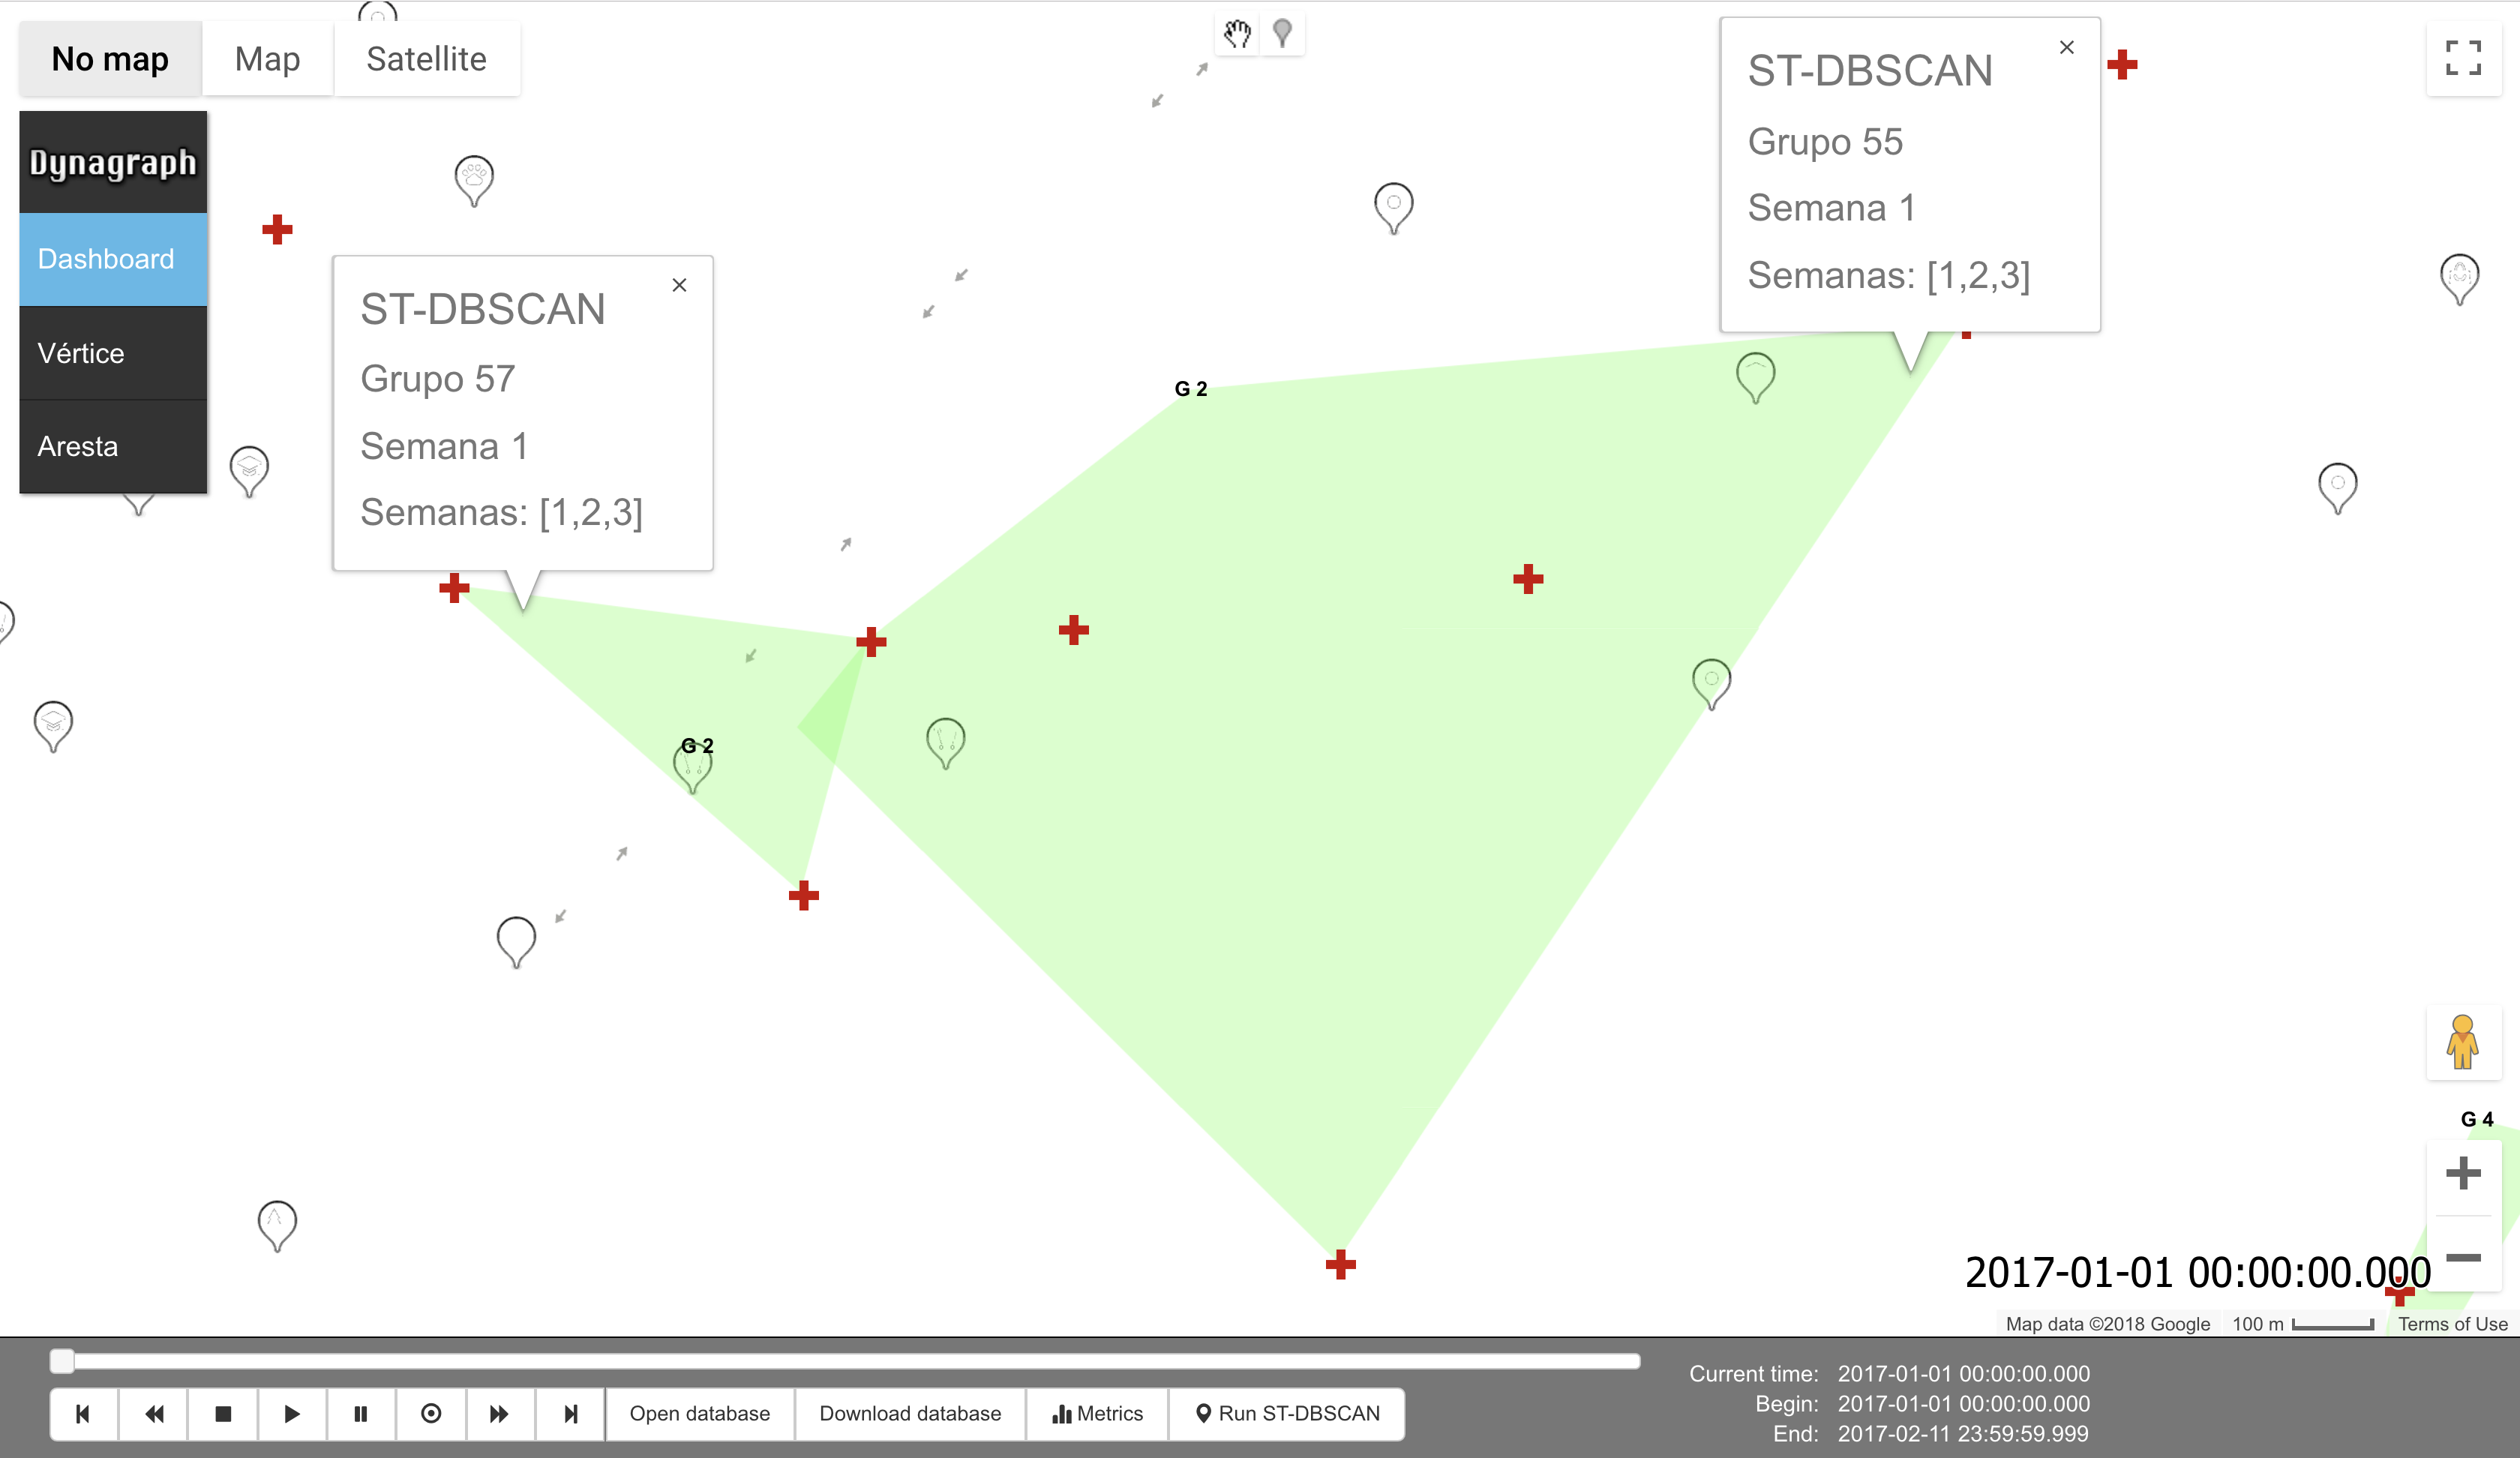
\includegraphics[width=15cm]{figuras/stdbscan/stdbscan1.png}
	}{
		\Fonte{Elaborado pelo autor}
	}
\end{figure}
\FloatBarrier

\begin{figure}[!ht]
	\centering	
	\Caption{\label{fig:stdbscan2} \acrshort{ST-DBSCAN}: Semana 2}
	\UECEfig{}{
		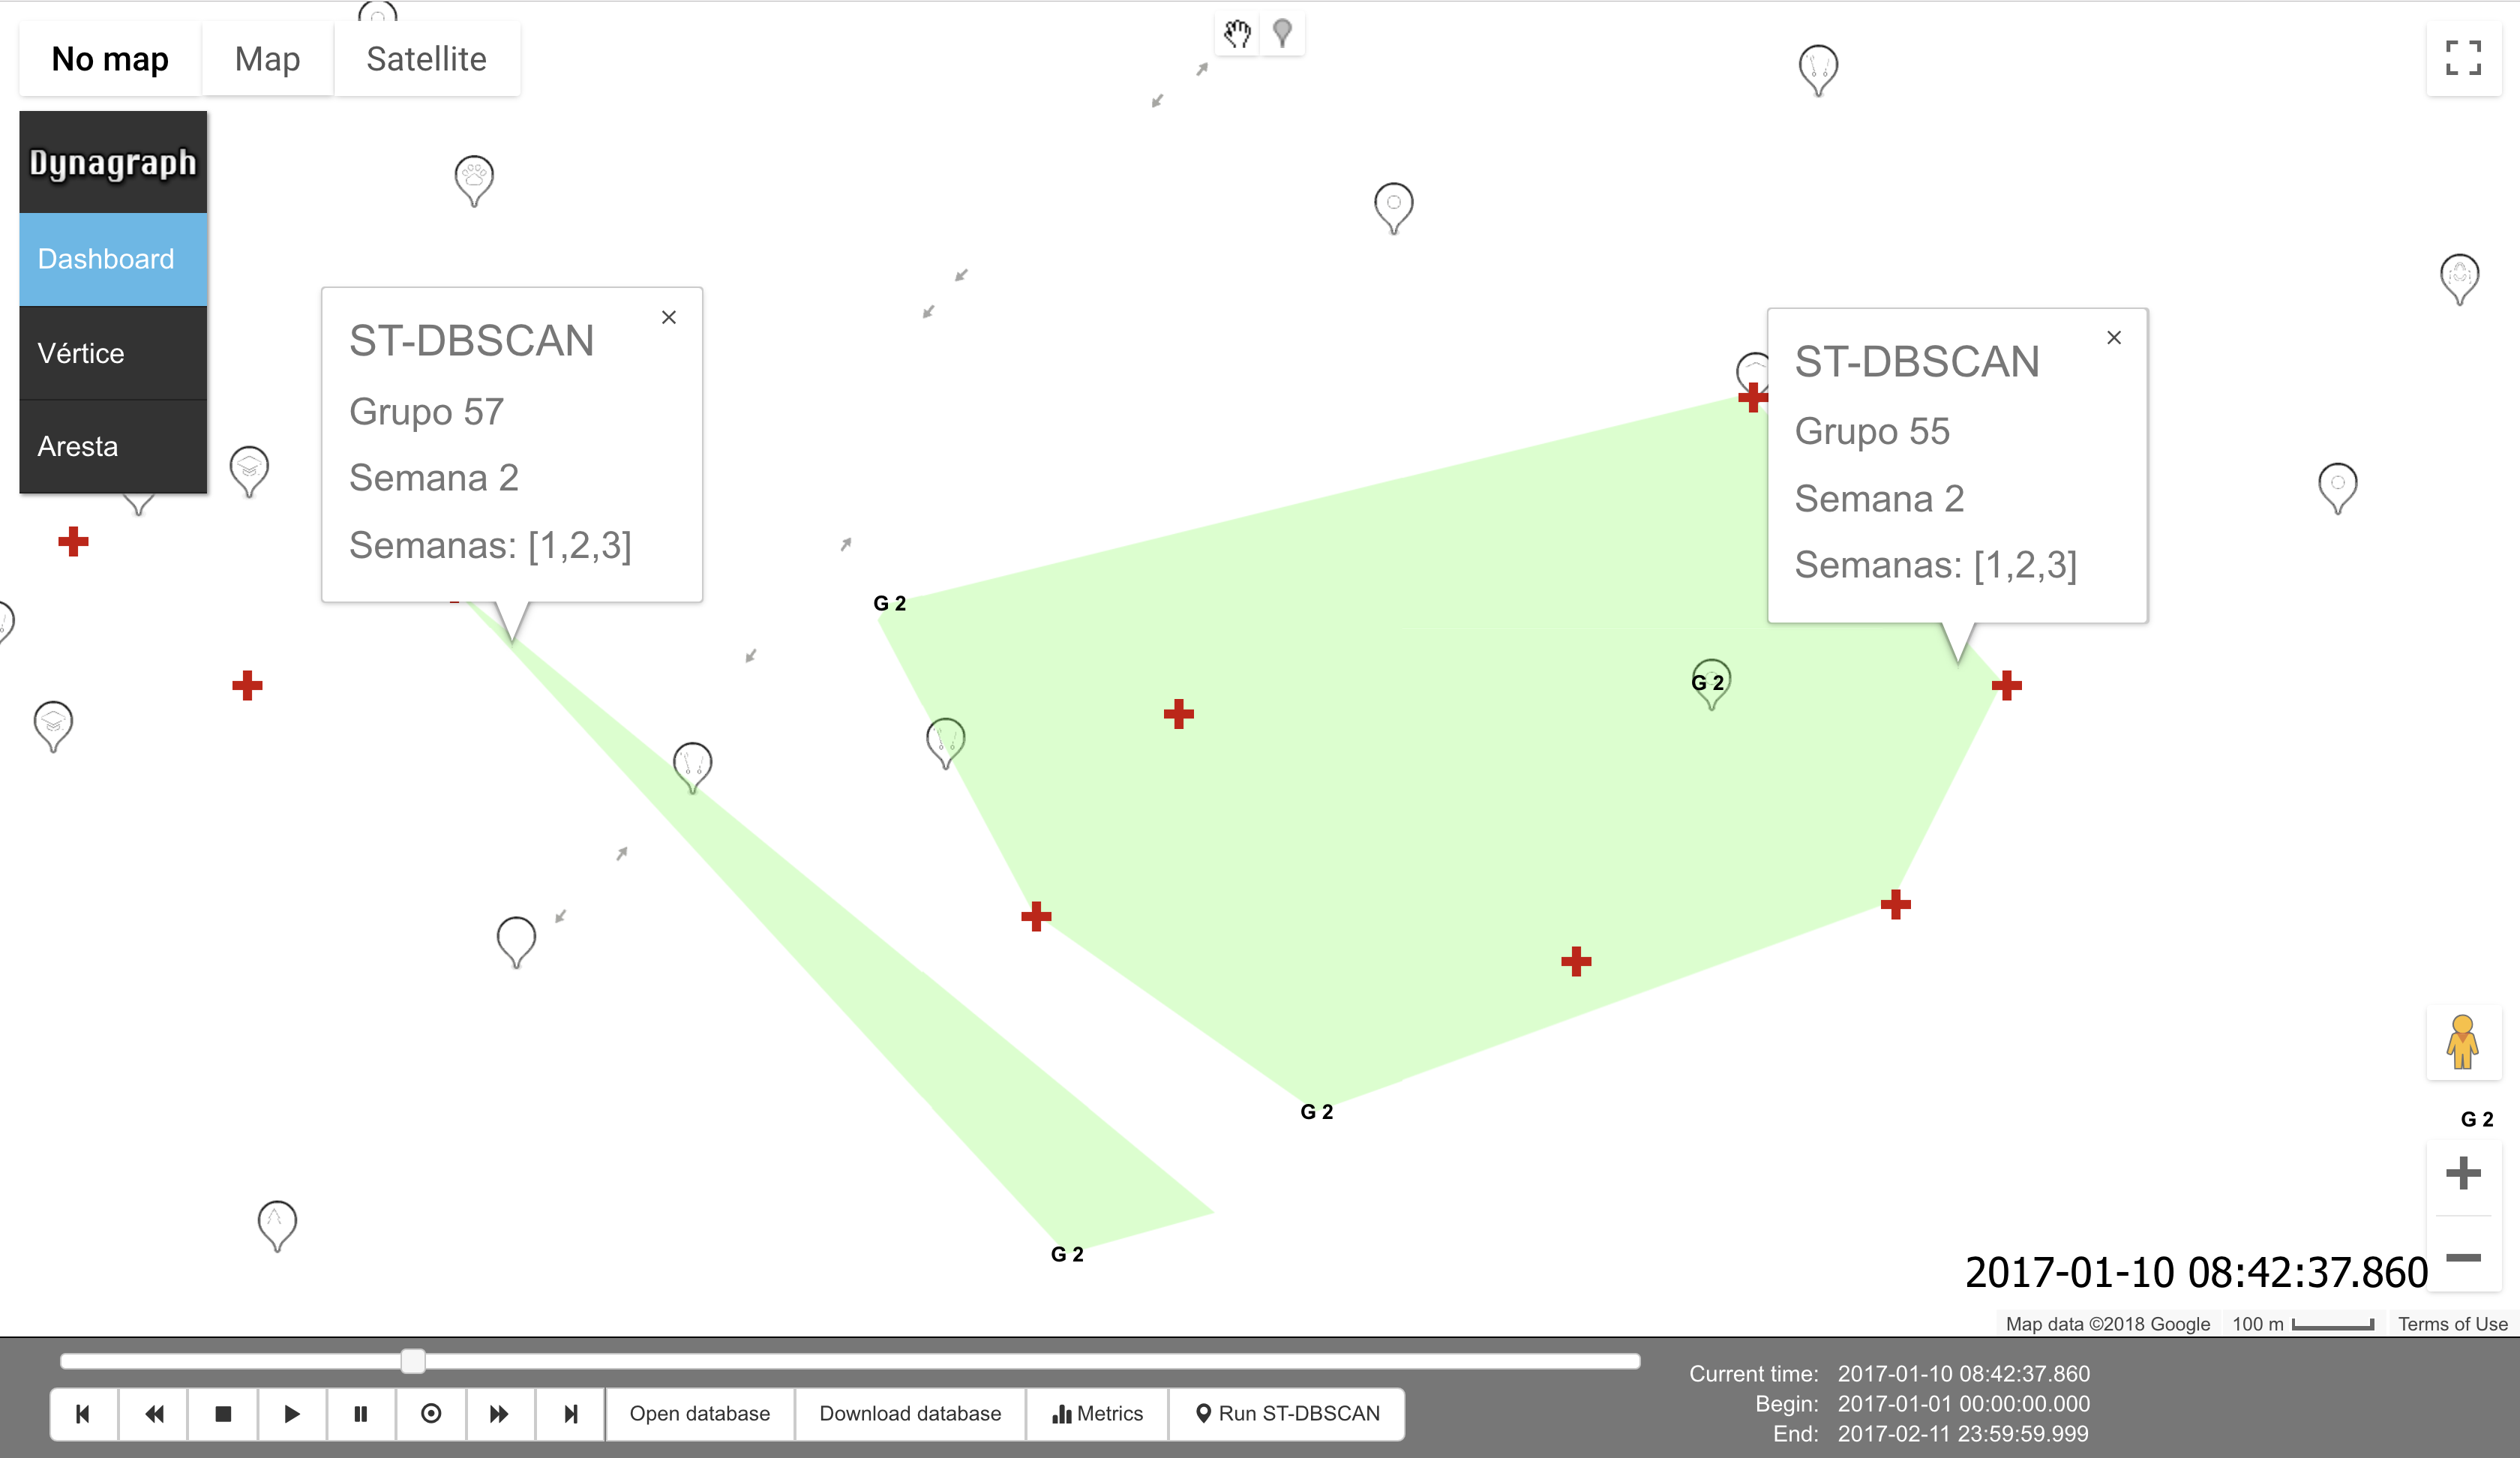
\includegraphics[width=15cm]{figuras/stdbscan/stdbscan2.png}
	}{
		\Fonte{Elaborado pelo autor}
	}
\end{figure}
\FloatBarrier

\begin{figure}[!ht]
	\centering	
	\Caption{\label{fig:stdbscan3} \acrshort{ST-DBSCAN}: Semana 3}
	\UECEfig{}{
		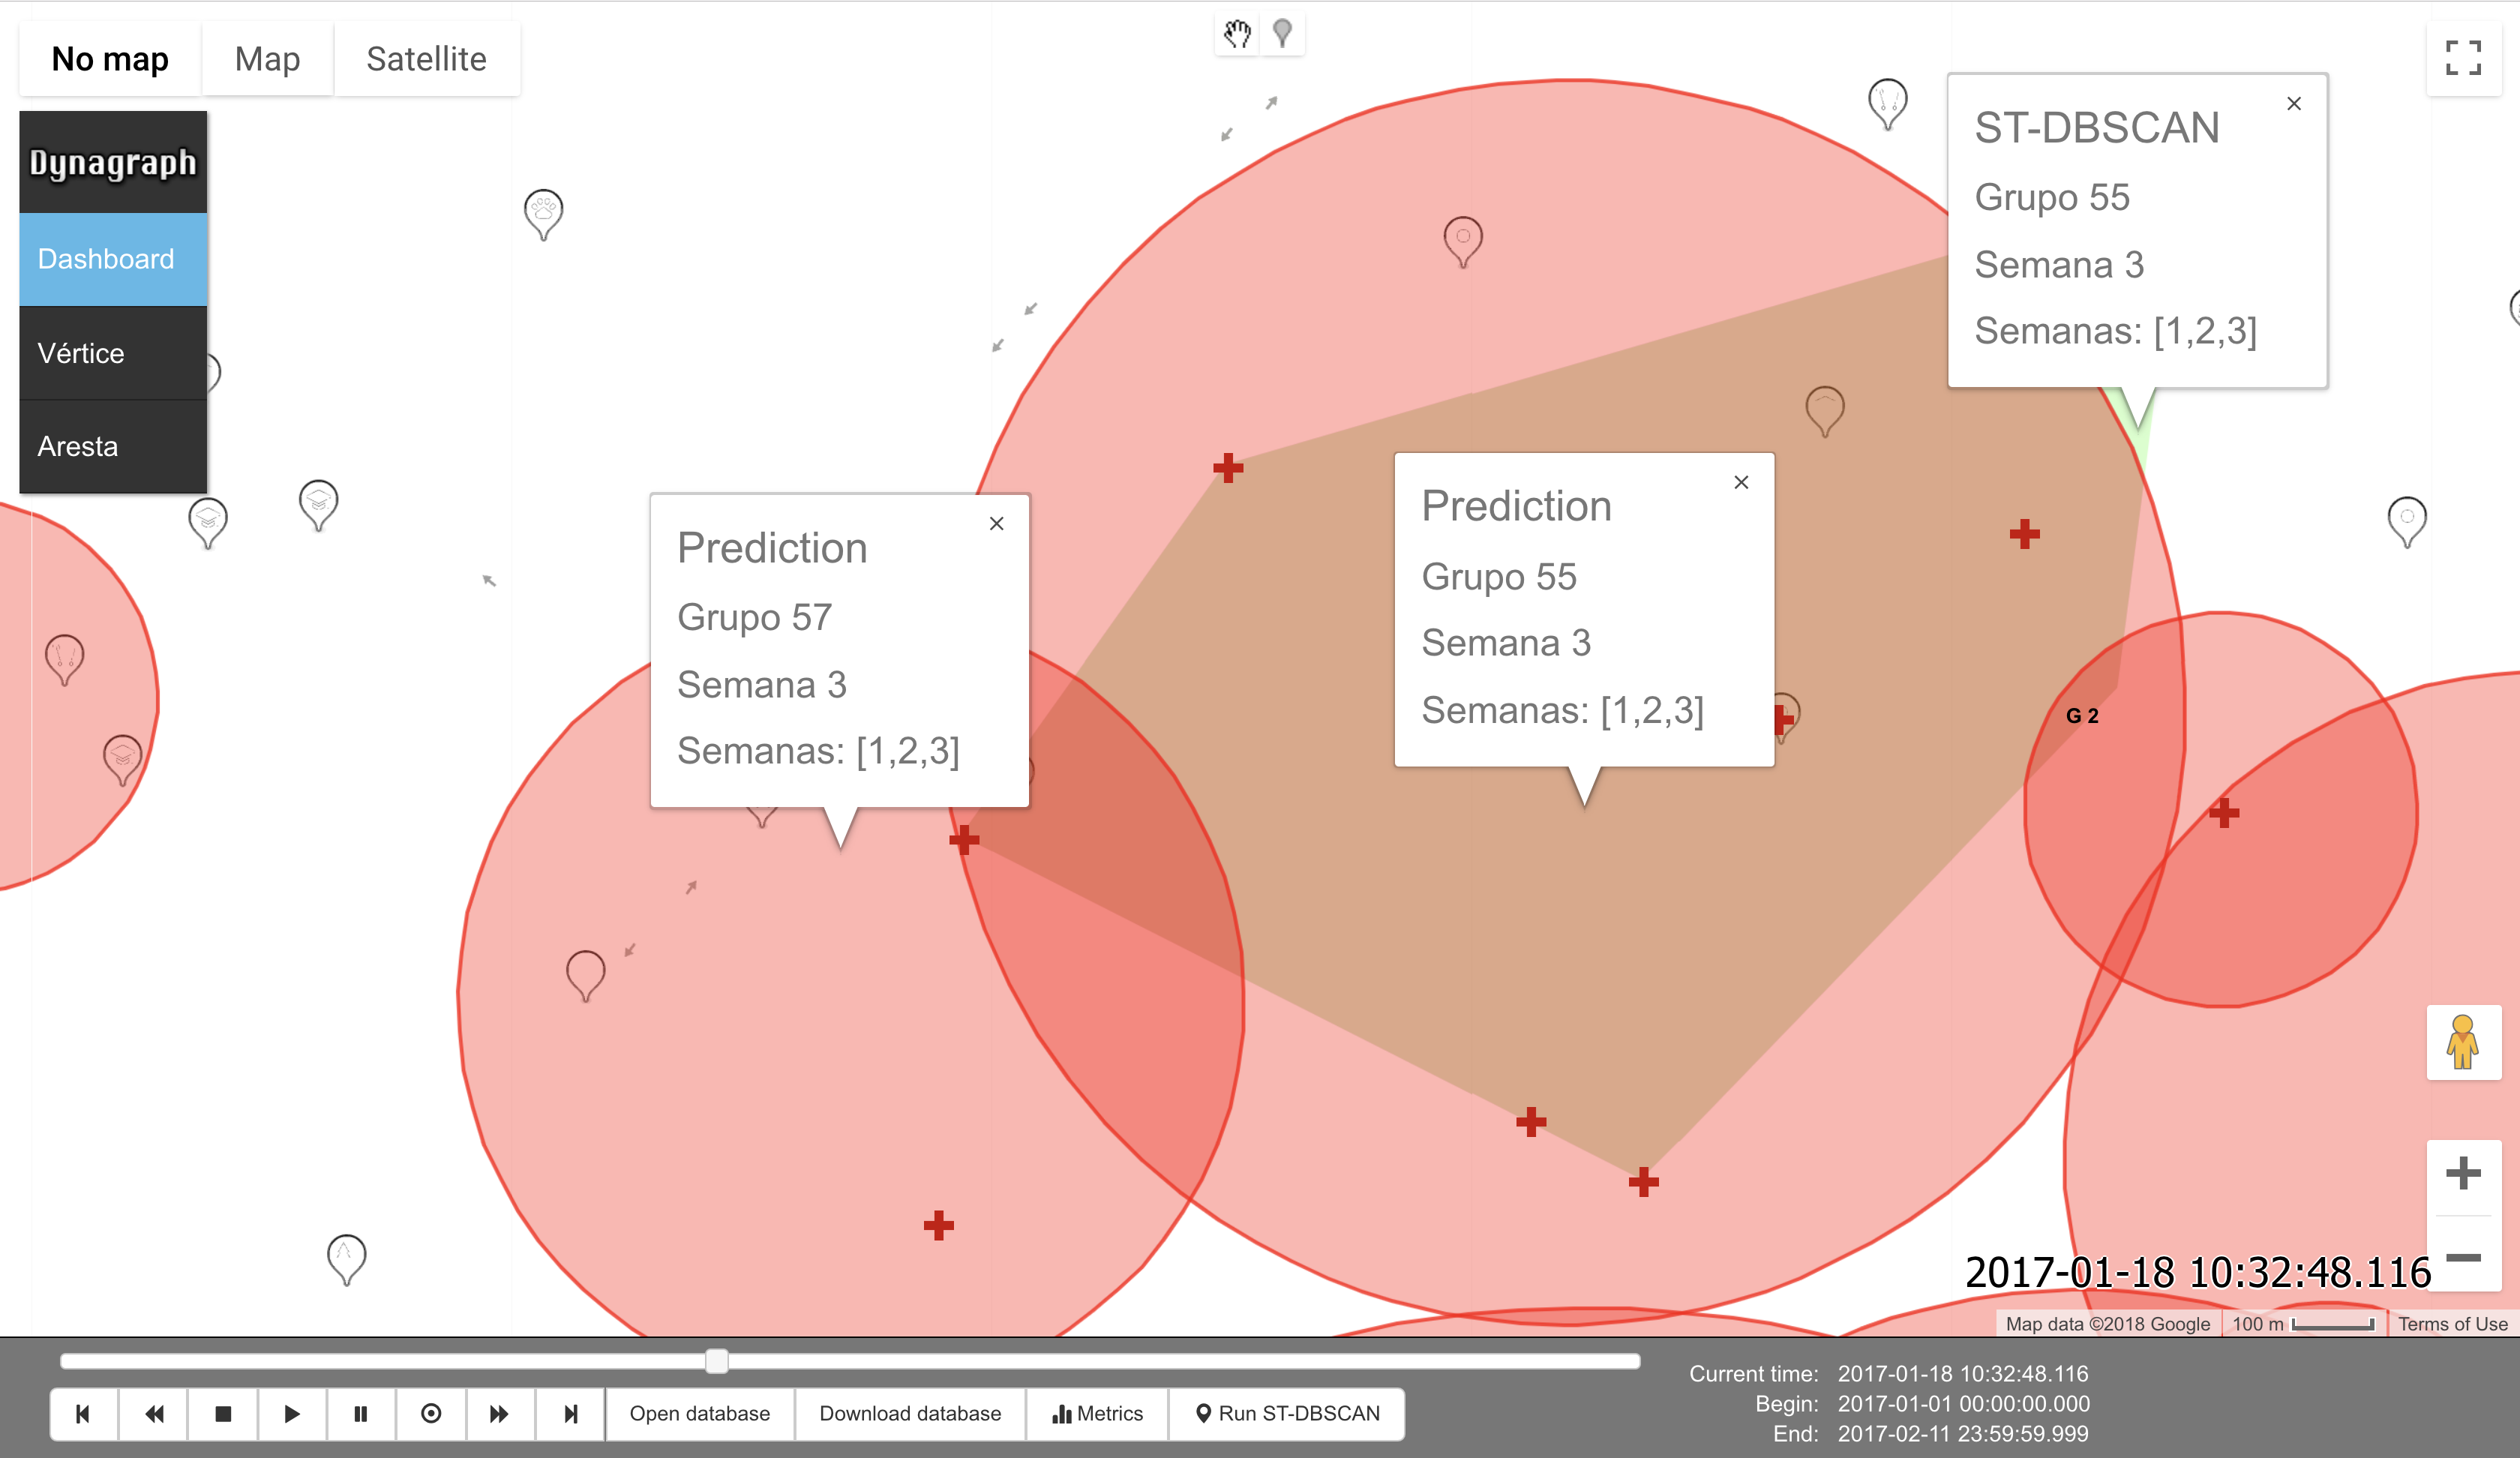
\includegraphics[width=15cm]{figuras/stdbscan/stdbscan3.png}
	}{
		\Fonte{Elaborado pelo autor}
	}
\end{figure}
\FloatBarrier
